% !TEX root = ../thesis.tex
% ==============================================================================
%  CHAPTER 4: PROPOSED METHODOLOGY (فصل چهارم: روش‌شناسی پیشنهادی) 
%             (chapters/chapter4_methodology.tex)
% ==============================================================================
%  This chapter details the theoretical formulation, architectural design,
%  and algorithmic pipeline of the proposed framework.
% ==============================================================================


\chapter{روش‌شناسی پیشنهادی}\label{chap:chapter4_methodology}

فصل چهارم پایان‌نامه به تشریح دقیق و گام‌به‌گام نوآوری و روش پیشنهادی نویسنده اختصاص دارد. در این فصل، رهیافت ارائه‌شده برای حل مسئله با تکیه بر فرمول‌بندی ریاضی، معماری سامانه و مراحل الگوریتمی تبیین می‌گردد. تمرکز اصلی باید بر وضوح فنی و دقت علمی باشد، به‌گونه‌ای که پژوهشگری دیگر با مطالعه‌ی متن بتواند روش را پیاده‌سازی و نتایج را بازتولید نماید.

در این قالب، فصل چهارم علاوه بر تبیین ساختار روش‌شناسی، دو قابلیت مهم حروف‌چینی را به نمایش می‌گذارد: بارگذاری تصاویر برداری خارجی (\lr{PDF}) و تنظیم شبه‌کدهای فنی با بسته \lr{algorithmicx} همراه با کلیدواژه‌های فارسی‌شده.


\section{معماری کلی سامانه و دیاگرام ساختاری}\label{sec:4-1}

در آغاز تشریح روش‌شناسی، ارائه‌ی یک دیاگرام ساختاری جامع از جریان داده‌ها و ارتباط میان لایه‌های سامانه به درک کلی روش کمک می‌کند. چنانچه نمودارها در نرم‌افزارهای خارجی (مانند \lr{Visio}، \lr{Illustrator}، \lr{Draw.io} یا خروجی پایتون) طراحی می‌شوند، ضروری است خروجی به‌صورت فایل برداری \lr{PDF} ذخیره و سپس با دستور \code{{\textbackslash}includegraphics} درج گردد. استفاده از قالب‌های پیکسلی (\lr{PNG} یا \lr{JPG}) موجب افت وضوح در چاپ و تار شدن خطوط در بزرگ‌نمایی می‌شود، در حالی که قالب برداری کیفیت نمادها و خطوط را در تمام مقیاس‌ها به‌طور کامل حفظ می‌کند.

در شکل~\ref{fig:chap4_architecture}، نمونه‌ای از معماری سه‌لایه‌ای سامانه که به‌صورت فایل \lr{PDF} برداری آماده و فراخوانی شده، نمایش داده شده است.

\begin{figure}[!ht]
    \centering
    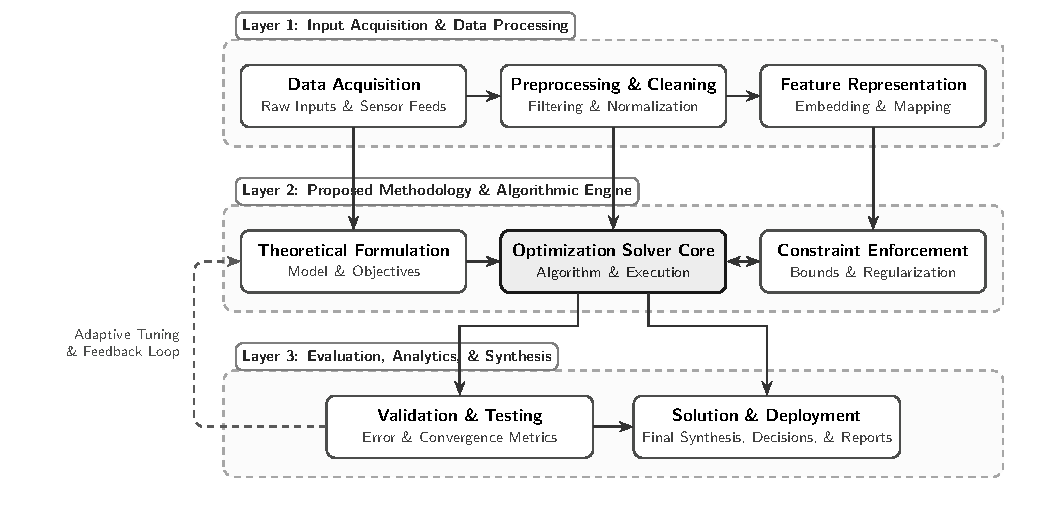
\includegraphics[width=\textwidth]{figures/fig_architecture.pdf}
    \caption{معماری ساختاری سامانه و چارچوب مفهومی لایه‌های روش‌شناسی پیشنهادی}\label{fig:chap4_architecture}
\end{figure}


\section{فرمول‌بندی نظری و مدل‌سازی ریاضی}\label{sec:4-2}

در ادامه‌ی متن فصل، اجزای روش پیشنهادی در بخشی مجزا و یا در امتداد هر زیربخش طرح، به زبان ریاضی مدل‌سازی می‌شوند. فرض کنید بردار ورودی $\mathbf{x} \in \mathbb{R}^d$ با استفاده از نگاشت پارامتری $f_\theta: \mathbb{R}^d \to \mathbb{R}^m$ به فضای ویژگی‌ها منتقل شود. برای دستیابی به توازن بهینه میان دقت و پایداری سامانه، تابع هدف پیشنهادی به‌صورت مسئله‌ی بهینه‌سازی مقید زیر صورت‌بندی می‌شود:
\begin{equation}\label{eq:chap4_objective}
    \begin{aligned}
        \min_{\theta} \quad \mathcal{L}(f_\theta(\mathbf{x}), \mathbf{y}) + \lambda_1 \, \|\theta\|_1 + \frac{\lambda_2}{2} \, \|\theta\|_2^2 \qquad \text{s.t.} \quad \mathbf{c}(\theta) \le \mathbf{0}
    \end{aligned}
\end{equation}
در معادله‌ی~\eqref{eq:chap4_objective}، عبارت اول بیانگر تابع زیان عملکردی نسبت به خروجی مطلوب $\mathbf{y}$، دو جمله‌ی بعدی منظم‌سازهای نُرم اول و دوم برای کنترل پیچیدگی پارامترها، و $\mathbf{c}(\theta)$ بیانگر قیدهای فیزیکی یا ساختاری سامانه است.


\section{شبه‌کد الگوریتم و مراحل اجرایی}\label{sec:4-3}

ارائه‌ی شبه‌کد دقیق از مراحل آموزش، پردازش یا استنتاج روش، شفافیت عملیاتی آن را تضمین می‌کند. در این قالب، محیط \lr{algorithmicx} برای نگارش الگوریتم‌ها با قابلیت شماره‌گذاری خطوط و ترجمه‌ی فارسی دستورها (شامل «ورودی»، «خروجی»، «به ازای»، «اگر» و «برگردان») آماده‌سازی شده است. در الگوریتم~\ref{algo:chap4_training}، روند اجرایی روش پیشنهادی خلاصه شده است.

\begin{algorithm}[!ht]
\caption{روند محاسباتی و مراحل بهینه‌سازی روش پیشنهادی}\label{algo:chap4_training}
\begin{algorithmic}[1]
\vspace{0.15cm}
\Require{مجموعه‌داده‌ی ورودی $\mathcal{D}$، نرخ یادگیری $\eta$، آستانه‌ی همگرایی $\epsilon$}
\Ensure{بردار پارامترهای بهینه‌شده‌ی $\theta^*$}
\vspace{0.25cm}
\State{مقداردهی اولیه‌ی پارامترها $\theta^{(0)}$ و شمارنده‌ی تکرار $k \leftarrow 0$}
\vspace{0.15cm}
\While{معیار توقف برآورده نشده است}
    \State{انتخاب دسته‌ی نمونه‌های داده $\mathcal{B} \subset \mathcal{D}$}
    \State{محاسبه‌ی گرادیان تابع هدف: $\mathbf{g}^{(k)} \leftarrow \nabla_\theta \mathcal{L}(\theta^{(k)}; \mathcal{B})$}
    \State{به‌روزرسانی پارامترها: $\theta^{(k+1)} \leftarrow \theta^{(k)} - \eta \, \mathbf{g}^{(k)}$}
    \If{$\|\theta^{(k+1)} - \theta^{(k)}\|_2 < \epsilon$}
        \State{توقف حلقه و خروج}
    \EndIf{}
    \State{$k \leftarrow k + 1$}
\EndWhile{}
\vspace{0.15cm}
\State{\Return{$\theta^* \leftarrow \theta^{(k)}$}}
\vspace{0.15cm}
\end{algorithmic}
\end{algorithm}


\section{تحلیل پیچیدگی محاسباتی و منابع}\label{sec:4-4}

بخشی اساسی در بررسی علمی هر روش جدید، تحلیل پیچیدگی محاسباتی زمانی\enfootnote{time complexity} و حافظه‌ای\enfootnote{space complexity} آن است. در نگارش این بخش، باید نشان داده شود که روش پیشنهادی در مقایسه با گزینه‌های موجود، در چه مرتبه‌ای از مقیاس‌پذیری ($\mathcal{O}$) عمل می‌کند و آیا نیازمند منابع محاسباتی فراتر از استانداردهای متعارف است یا خیر. این تحلیل پیش‌درآمدی منطقی برای ورود به آزمون‌های تجربی در فصل پنجم خواهد بود.
